% Add a section on Implementation Issues, choice of libraries, language etc
% compare normalized vs non-normalized combination of kernels
% maybe compare our own validation technique, p-value graph, pvalue avg
\begin{quote} ``But since the affairs of men rest still incertain, Let's reason with the worst that may befall.'' - \textit{William Shakespeare (Julius Caesar)}\end{quote} 
\section{Introduction}
As we saw in the previous chapters, each of the current datasets, e.g. microarrays, DNA-binding, protein-protein interaction and sequence datasets, provide a partial and noisy picture of cell regulation. Hence, integration among these is required in order to obtain an improved picture of the underlying process. Initial methods of data integration in regulatory module discovery were mostly ad-hoc approaches that used clustering with some form of prior knowledge. Later on these were enhanced to incorporate model based clustering methods as well. One of the major drawbacks of these techniques was that they worked well on vectorial data but as soon as other types of data were encountered, the principled nature of the algorithms broke down and they had to resort to ad-hoc statistical techniques for finding correlations in datasets.

In the previous chapter we proposed a similarity based method which is very pertinent for non-vectorial data as there are established techniques to compute similarity from these. We will continue using similarity based techniques in this chapter. The bigger challenge that we saw in the last chapter was that of \textit{ad hoc} combination of datasets. Since they are reported as p-values, the DNA-binding data could be interpreted as similarity values. The similarity values in the DNA-binding dataset were converted into constraints and then combined to the microarray data using \textit{ad hoc} p-value thresholds. In order to do the integration in a \textit{principled} manner, we needed a framework under which various types of data could be integrated and their effects analyzed. Various earlier researchers have used the Bayesian framework for merging data, but in our opinion it is unsuitable to cope with non-vectorial data (strings, graphs) in a principled manner as it was primarily developed for vectorial data. 

To summarise, the problem now is reduced to having two similarity matrices and we need some method to integrate them. A simpler approach to integrating matrices is the \textit{shrinkage} method. When there are two similarity matrices $K_{1} and K_{2}$, a final combination $K$ could be written as,
\begin{eqnarray}
K &=& \mu K_{1}+(1-\mu)K_{2}
\end{eqnarray}
which represents a \textit{convex combination}\footnote{A convex combination is a linear combination of where all coefficients are non-negative and sum up to 1} of $K_{1}$ and $K_{2}$ with the shrinkage parameter $\mu$ ranging between 0 and 1, and controlling what fraction of each similarity matrix contributes towards the final matrix. The \textit{shrinkage} method is named so because depending on the $\mu$, we shrink the contribution of the original evidence. For example, if we are combining microarray data with \ac{PPI} data to improve the predictions based just on microarray data, then the contribution of microarray data is being shrunk from its original contribution (which is 1). Optimum $\mu$ values can be chosen after running these various weight combinations of datasets through the Spectral clustering algorithm and then optimizing for the best cluster quality using the Dunn or Davies-Bouldin index values. While this is reasonable from a practical viewpoint, its not very principled. That motivates us towards our next step which is to use the principle of maximum entropy (Section-\ref{kern_integration}) in order to merge the similarity matrices. As we will see in following sections, this allows us to merge two datasets when there is no evidence available regarding their individual importance. For example, when we have two noisy data sources e.g. microarray and \ac{PPI}, and no other evidence regarding their individual importance, we can combine them to get better inference using the principle of maximum entropy.

As discussed in Section-\ref{kern_integration}, we need a more specialised version of the similarity matrix for maximum entropy integration. The extra requirement is that our similarity matrices should be positive semi-definite. There is a separate but similar branch of machine learning that operates only on such matrices and are known as \textit{kernel methods}. We describe them in Section-\ref{kern_methods}. Throughout this chapter, we have used similarity matrices, kernels and kernel matrices interchangeably to refer to \textit{positive semi-definite symmetric similarity matrices}.

\section{Elementary Linear Algebra} \label{maxent:linalg}
In this section we describe some of the basic principles of Linear Algebra. It is only a concise introduction for the purpose of explaining terminology used in this chapter. More details can be found in any standard text on the topic like \citet{Strang2006Linear, golub1996matrix}.
\subsection{Vectors and matrices}
In the context of linear algebra, a vector is a linearly ordered set of real numbers and is usually denoted by a lowercase boldface letter, e.g. $\mathbf{v}$. The numbers are the components of the vector. They are represented in a columnar form. The number of components determine the \textit{dimension} of the vector. We say that $\mathbf{v}$ is an $n$ dimensional vector, or a point in the $n$ dimensional real number space ($\mathbf{v} \in \mathbb{R}^{n}$).
\textit{Transpose} of a vector is the row-wise representation of a column vector or \textit{vice versa}, and is denoted by a superscripted boldface lowercase letter, e.g. $\mathbf{{v}^{T}}$. 

A \textit{matrix} is a rectangular array of numbers characterized by the number of rows and columns. It is usually denoted by a boldface capital letter, e.g. $\mathbf{A}$ and its elements by corresponding lowercase letter with subscripts for row and column numbers, e.g. $a_{ij}$. If $\mathbf{A}$ has m rows and n columns, we say that it is an element of the $m \times n$ dimensional space of real numbers ($\mathbf{A} \in \mathbb{R}^{m \times n}$). If $m=n$ then the matrix is called a \textit{square} matrix. The \textit{transpose} of a $m \times n$ matrix $\mathbf{A}$ is denoted by $\mathbf{A}^{T}$ and is a $n \times m$ matrix which is obtained by interchanging the rows and columns of $\mathbf{A}$. A matrix is known to be \textit{symmetric} if $\mathbf{A}=\mathbf{A}^{T}$ which requires that the matrix is square and $a_{ij}=a_{ji}$.

The product of a matrix $\mathbf{A}$ and a vector $\mathbf{x}$, $\mathbf{Ax}$ is defined if $\mathbf{A} \in \mathbb{R}^{m \times n}$ and $\mathbf{x} \in \mathbb{R}^{n}$. In other words, this product is possible if the column dimension of $\mathbf{A}$ is same as the dimension of $\mathbf{x}$. The final result of this product is an $m$ dimensional vector. We can state this in words as: $m \times n$ dimensional matrix $\mathbf{A}$ transforms the n dimensional vector $\mathbf{x}$ into an m dimensional vector when multiplied to it.

A matrix is \textit{diagonal} if all its off-diagonal elements are zero. If $\mathbf{D}$ is a square diagonal matrix it can be defined by the list of its diagonal elements, $\mathbf{D}=diag(d_{i})$. The \textit{unit matrix} is a special case of a square diagonal matrix where all the diagonal elements are 1. It is denoted by $\mathbf{I}$ or $\mathbf{I_{m}}$ where m is the dimension. Any multiplication by a unit matrix (pre or post) to a conformable (the dimensions are such that the multiplication is possible) matrix $\mathbf{A}$ results in $\mathbf{A}$.

The \textit{column rank} of a matrix is the maximum number of linearly independent columns in that matrix. Similarly, the \textit{row rank} of a matrix is the maximum number of linearly independent rows in that matrix. Row and column ranks are always equal and is referred to simply as the \textit{rank} of the matrix. A matrix whose columns are linearly independent is said to have \textit{full column rank}. Similarly, a matrix whose rows are linearly independent is said to have \textit{full row rank}. The matrix is said to have \textit{full rank} if it has either full column rank or full row rank. If the rank of the matrix is less than the full rank then it is known as \textit{rank-deficient} matrix.
 
A square matrix with linearly independent columns is termed as \textit{non-singular}. If the columns are linearly dependent it is \textit{singular}. For every non-singular matrix $\mathbf{A}$ there exists an associated matrix $\mathbf{A}^{-1}$ known as its inverse or simply $\mathbf{A}$ \textit{inverse} such that
\begin{displaymath}
    \mathbf{A}^{-1}\mathbf{A} = \mathbf{I}
\end{displaymath}
Since an inverse exists for all non-singular matrices they are \textit{invertible}.

\subsection{Eigenvalues and eigenvectors} \label{eigval_eigvec}
For every square matrix $\mathbf{A}$, there exists at least one number $\lambda$ and an associated non-zero vector $\mathbf{u}$ such that 
\begin{eqnarray}
    \mathbf{Au} = \lambda \mathbf{u} \label{eqn:eigenvec_eigenval}
\end{eqnarray}
Thus, matrix $\mathbf{A}$ does not change the direction of $\mathbf{u}$. A value of $\lambda$ for which Equation-\ref{eqn:eigenvec_eigenval} holds true is known as the \textit{eigenvalue} of $\mathbf{A}$ and the corresponding vector is known as the \textit{eigenvector} of $\mathbf{A}$. Eigenvalues, in the general case, could also be complex numbers but symmetric matrices have real eigenvalues. The eigenvalues and eigenvectors of a matrix together are known as the \textit{eigensystem} of that matrix.

The sum of the diagonal elements of a square matrix $\mathbf{A}$ is known as the \textit{trace} of $\mathbf{A}$. It is also equal to the sum of the eigenvalues.  
\begin{displaymath}
    trace(\mathbf{A}) = \sum_{i=1}^{m}a_{ii}=\sum_{i=1}^{m}\lambda_{i}(\mathbf{A}) 
\end{displaymath}
The product of the eigenvalues is equal to the \textit{determinant} of $\mathbf{A}$.
\begin{displaymath}
    det(\mathbf{A}) = \prod_{i=1}^{m}\lambda_{i}(\mathbf{A}) 
\end{displaymath}

\subsection{Spectral or eigen-decomposition}
Spectral or eigen decomposition of a symmetric $n \times n$ matrix $\mathbf{A}$ is represented as
\begin{displaymath}
    \mathbf{A} = \mathbf{Q} \Lambda \mathbf{Q}^{-1}  
\end{displaymath}
where $\Lambda = diag(\lambda_{i})$ is the diagonal matrix, $\lambda_{i}$'s are the eigenvalues of $\mathbf{A}$ and $\mathbf{Q}=[q_{1},\dots,q_{n}]$ is the square $n \times n$ matrix whose $i_{th}$ column is the basis eigenvector $q_{i}$ of $\mathbf{A}$.
  
A symmetric matrix $\mathbf{A}$ is said to be \textit{positive definite} if
\begin{displaymath}
    \mathbf{x}^{T}\mathbf{A}\mathbf{x} > 0 \mbox{ for all non-zero x}  
\end{displaymath}

A symmetric matrix $\mathbf{A}$ is said to be \textit{positive semi-definite} if
\begin{displaymath}
    \mathbf{x}^{T}\mathbf{A}\mathbf{x} \geq 0 \mbox{ for all non-zero x}  
\end{displaymath}
All the eigenvalues of a positive definite matrix are positive whereas the eigenvalues of a positive semi-definite matrix are non-negative.  

\section{Kernel Methods} \label{kern_methods}

\textit{Kernel methods} are algorithms that operate on a type of data representation known as a \textit{kernel} matrix. Kernel matrices provide a general framework to represent data and satisfy certain mathematical properties. A kernel matrix is defined not in terms of individual variables but in terms of pairwise similarity among all variables. So, instead of using a mapping $\phi:\mathcal{X}\rightarrow\mathcal{F}$ to represent each object $\mathbf{x}\in\mathcal{X}$ by $\phi(\mathbf{x})\in \mathcal{F}$, a real valued similarity function $k:\mathcal{X} \times\mathcal{X}\rightarrow\mathbb{R}$  is used and the dataset with n variables is represented by a n $\times$ n matrix of pairwise similarities $k_{ij}=k(\mathbf{x}_{i},\mathbf{x}_{j})$. The most significant fact regarding these methods is that once we have a kernel matrix representation of the data then the original data is not required and the methods can work on just these matrices. This is where the real beauty of these methods arise as different types of data types do not necessitate changes in the underlying algorithm. Kernel methods require that a kernel matrix is \textit{symmetric} and \textit{positive semi-definite}. This means that if $k$ is an $n \times n$ matrix of pairwise similarities then $k_{i,j}=k_{j,i}$ for $1 \leq i,j \leq n$, and $\mathbf{c}^\top k \mathbf{c} \geq 0$ for any $c \in \mathbb{R}^{n}$. This also implies that the matrix has non-negative real eigenvalues. 

Each similarity value ($k_{i,j}$) in a kernel matrix is calculated using a so called kernel function ( k(x,y) ) that acts a \textit{suitable} similarity between the variables. Hence, a real valued kernel matrix could be obtained for diverse data types (strings and graphs) as long as a similarity function can be defined over a pair. This nice property leads to complete separation of similarity function definition from the algorithms that operate on these matrices. This is specially useful in bioinformatics because of diverse types of datasets (as pointed in previous chapter) where a real valued representation of individual variables is non intuitive while a similarity score makes sense, e.g. genomic sequences. We will see different types of kernels in Section-\ref{kern_types}. 

\subsection{Various kernel or similarity functions}\label{kern_types}
We provide a short description of various possible kernels for different data types (vectors, strings and graphs) and their properties.

\subsubsection{Vector Data}
\begin{itemize}
 \item The \textit{Linear} or \textit{Dot kernel} is the simplest one.
\begin{equation}
 k_{L}(\textbf{x},\textbf{x}^{'})=\textbf{x}^{T}\textbf{x}^{'}
\end{equation} 
 \item The \textit{Polynomial kernel} is a more general case of the linear kernel
\begin{equation}
 k_{Poly}(\textbf{x},\textbf{x}^{'})=(\textbf{x}^{T}\textbf{x}^{'}+c)^d
\end{equation} 
where d is the degree of the polynomial and c is a constant. When c is non-zero then this kernel corresponds to a feature space spanned by all products of at most 2 variables i.e., ${\lbrace 1,x_{1},x_{2},x_{1}^{2},x_{1}x_{2},x_{2}^{2} \rbrace}$. When c is zero then this space is restricted to only the products of exactly 2 variables i.e., ${\lbrace x_{1}^{2},x_{1}x_{2},x_{2}^{2} \rbrace}$.
 \item The most popular and widely used kernel function used for real data is the \textit{Gaussian} or \textit{Radial Basis Function (RBF) kernel}
\begin{equation}
 k_{G}(\textbf{x},\textbf{x}^{'})=exp \left( -\frac{{\parallel \textbf{x}-\textbf{x}^{'} \parallel}^{2}}{2\sigma^{2}}\right)
\end{equation}
the width of the Gaussian being controlled using $\sigma$. This affinity function naturally encodes the local neighbourhood property and its value falls rapidly as the pairwise dissimilarity increases.
\item Another popularly used kernel is the \textit{Sigmoid kernel}

\begin{equation}
 k_{S}(\textbf{x},\textbf{x}^{'})=(k\textbf{x}^{T}\textbf{x}^{'}+\theta) 
\end{equation}
where $k>0$ and $\theta < 0$ are the \textit{gain} and \textit{threshold}. 

\end{itemize}

\subsubsection{Graph data}
A graph is informally defined as a set of \textit{nodes} connected by \textit{edges}. In bioinformatics, typical examples of a graph would be the interactions between the proteins of an organism or the interaction network representing the metabolic pathway. Other common examples of such graphs are social networks and hyperlinked internet web pages. While a graph represents \textit{local similarity} i.e., a node's direct interactions in its neighbourhood, we need a similarity function that represents \textit{global similarity} i.e., a node's interaction to every other node in the graph. The simplest measure of similarity on a graph is the shortest-path distance, but it is not positive semi-definite which is our requirement. Apart from this, this is very sensitive to insertions and deletions of edges. A more robust similarity measure is required which could perhaps average over many paths. The physical process of diffusion suggests a natural way of propagating such local information and has led to the most popular type of similarity on graphs known as the \textit{diffusion} kernel \citep{Kondor02diffusion}.

Laplacian $L$ of an \textit{undirected unweighted} graph is defined as,
\begin{eqnarray}
L_{i,j} &=& \begin{cases}
             -1 & \text{for i $\sim$ j,} \\
	     d_{i} & \text{for i=j,} \\
	     0 & \text{otherwise}
            \end{cases}
\end{eqnarray}
where $i \sim j$ implies that $i$ and $j$ are connected by an edge and $d_{i}$ is the number of edges originating from $i_{th}$ node. The kernel function on the graph can be defined using the negative of this Laplacian ($H=-L$) as
\begin{eqnarray}
K_{\beta} = e^{\beta H}= \lim_{m->\infty}\big ( \mathbf{I}+\frac{\beta H}{m}\big )^m
\end{eqnarray}
where $\beta$ is a positive constant and $\mathbf{I}$ is an identity matrix. $K_{\beta}$ represents an exponential family of similarity functions with generator $H$ and bandwidth parameter $\beta$. Using power series expansion this can be expanded to
\begin{eqnarray}
K_{\beta}=  \mathbf{I}+ \beta H +\frac{\beta ^2 H^2}{2} +\frac{\beta ^3 H^3}{3!} + \dots \label{diffusion}
\end{eqnarray}

Note that $e^{\beta H}$ yields a matrix but it is not the same as component-wise exponentiation $e^{\beta H_{ij}}$. If a matrix is diagonal then its exponential can be obtained by just exponentiating every entry on the diagonal, i.e., $e^{D}=diag(e^{d_{11}},e^{d_{22}},\dots,e^{d_{nn}})$. This is an important property that could be used for computing the exponential. If we diagonalise $H$ i.e., if $H = UDU^{-1}$ and D is diagonal, then $e^{H} = Ue^{D}U^{-1}$. Based on this, we have used the technique discussed in \citet{Moler2003Nineteen} to compute our matrix exponentials. It involves computing the normalized eigenvalues and eigenvectors of $H$.
\begin{equation}
    H = \sum_{i=1}^{n}v_{i}\lambda_{i}v_{i}^{T}
\end{equation}
which when replaced in Equation-\ref{diffusion}
\begin{equation}
   K_{\beta}=\sum_{i=1}^{n}v_{i}e^{\beta \lambda_{i}}v_{i}^{T}
\end{equation}

This similarity function is also known as the \textit{diffusion} function because its differential equation form resembles the diffusion equation of heat through continuous media in classical physics \citep{Kondor02diffusion}. The function of $\beta$ is to control the extent of diffusion similar to the $\sigma$ of the Gaussian kernel. In fact, as shown in \citet{kernel_methodsvert2004}, there is straightforward correspondence between the diffusion kernel and the Gaussian kernel. The former can be considered a discretized version of the latter. In the next section we discuss our actual technique of similarity matrix integration. 

\subsection{From similarities to a valid kernel}
Sometimes we have a well defined measure of similarity between a pair of objects, but the resulting matrix is not a valid kernel matrix according to the strict definition of positive semi-definiteness. In such cases, two methods have been proposed in the literature that may be used to convert the similarity matrix to a valid kernel. \citet{tsuda99supportasymmetric} have proposed a principled technique called \textit{empirical kernel map}. \citet{roth2002going} have proposed an ad-hoc technique of eigen-decomposition of the similarity matrix and then removal of negative eigenvalues. They have also showed that this preserves the cluster structure of the data. When we are not sure if the similarity matrix that we have obtained is a kernel matrix then one of these techniques could be used to make it a kernel matrix. 
\subsection{Kernel normalization}
In order to add kernels, we need to normalize them so that they are on the same scale. Given an unnormalized kernel matrix, K, the normalized version is
\begin{equation}
    \hat{K_{ij}} = \frac{K_{ij}}{\sqrt{K_{ii} \times K_{jj}}}
\end{equation} 
This can be easily computed if we define $A = (1/\sqrt{K_{11}}, \dots, 1/\sqrt{K_{nn}})$. Then, $\hat{K} = K \ast (AA^{T})$, where $\ast$ denotes element-wise product.
 
\section{Principle of Maximum Entropy}
\subsection{Entropy} \label{information_theory}
While the term \textit{entropy} is popularly associated with thermodynamics, the entropy which we describe here comes from \textit{information theory}. This branch of applied mathematics and electrical engineering which deals with quantification of information was introduced by Claude E. Shannon in his seminal paper \citep{sha48mathematical}. While this original paper dealt with the engineering problem of the transmission of information over a noisy channel, the scope of information theory has widened a lot and touches subjects as diverse as cryptography to neurobiology. The most fundamental result of this theory is the \textit{source coding theorem}, according to which, on average, the number of bits needed to represent the result of an uncertain event is given by its \textit{entropy}. In other words, \textit{entropy} is a measure of the uncertainty associated with a random variable. 

If a discrete random variable $X$ takes values $x_{1}, \dots, x_{n}$ then its entropy $H$ is
\begin{displaymath}
    H(X) = E(I(X))
\end{displaymath}

where E is the expected value and I(X) is the \textit{information} content or \textit{self-information} of X. Now, if $p(x_i)$ is the probability of $X$ taking value $x_{i}$ then the entropy can explicitly be written as
\begin{displaymath}
    H(X) = \sum_{i=1}^n p(x_i)I(x_i) = -\sum_{i=1}^n p(x_i) \log_b p(x_i),
\end{displaymath}

where b denotes the base of the logarithm. The unit of entropy is the \textit{bit} or \textit{nat} for bases 2 and e respectively. If any of the probabilities vanish ($p(x_i) = 0$ for any $i$, we use the fact that $\lim_{p\to0}p\log p = 0$ and hence the value for that particular $i$ is zero. 

\textit{Differential entropy} also known as continuous entropy tries to extend the idea of Shannon entropy which is restricted to random variables taking discrete values to continuous probability distributions, e.g. Gaussian distribution. Another widely used measure of entropy for the continuous case is the \textit{relative entropy} of a distribution also popularly known as the KL divergence (refer Section-\ref{kl-divergence}). We will later maximize the differential entropy associated with a Gaussian distribution in order to merge similarity matrices (refer Section-\ref{kern_integration}). 


\subsection{Principle of maximum entropy} \label{maxent_principle}
Before we discuss our technique in detail, here we discuss the background and philosophical underpinnings of principle of maximum entropy. While in the earlier section we made a strict distinction between entropy associated to thermodynamics and information theory, at a more philosophical level, connections can be made between these two seemingly unrelated subjects. According to E.T. Jaynes in his seminal papers \citep{jaynes57maxent, jaynes82onrationale} 
\begin{quotation}
Thermodynamics should be seen as an application of information theory and the thermodynamic entropy is interpreted as being an estimate of the amount of further Shannon information needed to define the detailed microscopic state of the system, that remains uncommunicated by a description solely in terms of the macroscopic variables of classical thermodynamics. 
\end{quotation}
He proposed correspondence between statistical mechanics and information theory and suggested that the entropy in statistical mechanics, and the information entropy in information theory, are essentially the same thing. Consequently, statistical mechanics should be seen just as a particular application of a general tool of logical inference and information theory.

Suppose some testable information about a probability distribution is known. If we consider the set of all probability distributions which encode this information then the \textit{principle of maximum entropy (MaxEnt)} states that the probability distribution which maximizes the information entropy in view of the testable information is the true probability distribution. By choosing to use the distribution with the maximum entropy allowed by our information, we are choosing the most \textit{uninformative} distribution possible. If we choose any distribution with lower entropy then that would imply that we are assuming information which we do not have. On the other hand, if we choose a distribution with a higher entropy that would violate the constraints of the information we possess. Thus the maximum entropy distribution is the only reasonable distribution. Maximum entropy principles are used to choose the smoothest distributions out of all possible distributions. 

In our context, intuitively, each similarity matrix represents a distribution and we need to merge them so that the final distribution doesn't make assumptions about the individual weights of the matrices because that information is unavailable. We allow maximum entropy for the resulting distribution implying no assumptions whatsoever. This is the only approach available to us for kernel integration in the unsupervised domain.

Information theory as shown in Section-\ref{information_theory} defines \textit{information} in terms of probability distributions thus providing us with a quantitative measure of uncertainty (entropy) or ignorance. This can be maximized to find the maximally unbiased probability distribution. 

\section{Maximum Entropy Kernel Integration} \label{kern_integration}

We assume the \textit{similarity matrix} which is a symmetric positive semi-definite matrix to be the \textit{covariance matrix} of a \textit{Gaussian} distribution. Based on the earlier justification for the maximum entropy principle, we need to combine two similarity matrices such that the resulting one has maximum entropy. 

Now, a Gaussian distribution is represented as,
\begin{equation}
p(\mathbf{x|\mu,\Sigma})=\frac{1}{(2\pi)^{n/2}\lvert\Sigma\rvert^{1/2}}\exp \big\lbrace -\frac{1}{2}(\mathbf{x-\mu})^{T}\Sigma^{-1} (\mathbf{x-\mu}) \big \rbrace
\end{equation}
where $\lvert\Sigma\rvert$ is the determinant of the covariance matrix $\Sigma$, and $\mu$ is the mean of distribution. Its differential entropy is given by \citep{brookes2005matrix},
\begin{eqnarray}
H(p(\mathbf{x})) &=& -\int_{-\infty}^{+\infty} \int_{-\infty}^{+\infty} \dots \int_{-\infty}^{+\infty}p(\mathbf{x})ln (p(\mathbf{x})) d\mathbf{x} \\
&=& \frac{1}{2}(n+n ln(2\pi)+ln|\Sigma|) \label{diff_entropy_gauss}
\end{eqnarray}
In order to maximize $H(p(\mathbf{x}))$ we can ignore the first two terms ($n$ and $n ln(2\pi)$) in maximizing equation-\ref{diff_entropy_gauss} as they are constants. So, it becomes a problem of maximizing the $ln|\Sigma|$ term. We know that the determinant of a symmetric matrix is equal to the the product of its eigenvalues (refer Section-\ref{eigval_eigvec}), i.e.,
\[
|\Sigma|=\prod_{i=1}^{k}\lambda_{i}
\]
where $\lambda_{i}$ ($i=1\dots k$) are the $k$ eigenvalues of $\Sigma$. Therefore,
\begin{eqnarray}
ln|\Sigma|&=& ln\big (\prod_{i=1}^{k}\lambda_{i} \big) \\
&=& \sum_{i=1}^{k} ln (\lambda_{i}) \label{max_det}
\end{eqnarray}
Also, since logarithmic functions are monotonically increasing, so we can restate that \textit{in order to maximize the entropy of a Gaussian distribution, we need to maximize the $ln|\Sigma|$\footnote{this is also popularly known as log det maximization in optimization theory literature \citep{boyd2004convexopt}} which is equivalent to maximizing the sum of the eigenvalues of its covariance matrix}. Now assume that our covariance matrix is a combination of two covariance matrices and so can be rewritten as
\begin{eqnarray}
K &=& \sum_{i=1}^{2}\mu_{i}K_{i} \\
&=& \mu_{1}K_{1}+\mu_{2}K_{2}
\end{eqnarray}
where $\mu_{1}+\mu_{2}=1$. Now, according to spectral decomposition of a symmetric matrix,
\begin{eqnarray}
\Lambda &=& UKU^{T} \\ 
&=& U\big (\mu_{1}K_{1}+\mu_{2}K_{2} \big )U^{T} \\
&=& \mu_{1}UK_{1}U^{T}+\mu_{2}UK_{2}U^{T}  \\
&=& \mu_{1}Z_{1}+ \mu_{1}Z_{2} \label{eigv_split_1} 
\end{eqnarray}
where U is orthonormal and $\Lambda=diag[\lambda_{1},\lambda_{2},\dots,\lambda_{n}]$ is the diagonal matrix of eigenvalues. Matrices $Z_{1},Z_{2}$ are not diagonal matrices because U does not always diagonalises them. But, as U is the eigenvector matrix of the linear combination of $K_{1}$ and $K_{2}$, the off-diagonal elements of $Z_{1}$ and $Z_{2}$ cancel each other out \citep{thomaz2004covariance, carlos05maximum}. Therefore,
\begin{eqnarray}
\Lambda  &=& diag[\mu_{1}\lambda^{1}_{1},\mu_{1}\lambda^{1}_{2},\dots,\mu_{1}\lambda^{1}_{n}]+ diag[\mu_{2}\lambda^{2}_{1},\mu_{2}\lambda^{2}_{2},\dots,\mu_{2}\lambda^{2}_{n}] \label{eigv_split_2} \\
&=& diag[\mu_{1}\lambda^{1}_{1}+\mu_{2}\lambda^{2}_{1}, \mu_{1}\lambda^{1}_{2}+\mu_{2}\lambda^{2}_{2},\dots,\mu_{1}\lambda^{1}_{n}+\mu_{2}\lambda^{2}_{n}]  \\ 
%\lvert \Lambda \rvert &=& \prod_{i=1}^{n}{(\mu_{1}\lambda^{1}_{i}+\mu_{2}\lambda^{2}_{i})} \\
%ln \lvert \Lambda \rvert &=& \sum_{i=1}^{n}ln{(\mu_{1}\lambda^{1}_{i}+\mu_{2}\lambda^{2}_{i})}
\end{eqnarray}
where $\mu_{1}\lambda^{1}_{1},\mu_{1}\lambda^{1}_{2},\dots,\mu_{1}\lambda^{1}_{n}$ are the variance of $K_{1}$ spanned by the U eigenvector matrix and $\mu_{2}\lambda^{2}_{1},\mu_{2}\lambda^{2}_{2},\dots,\mu_{2}\lambda^{2}_{n}$ are the variance of $K_{2}$. In order to maximize the Eqn-\eqref{max_det}, we need to maximize the individual eigenvalues of the combined covariance matrix. So, effectively it implies that we need to maximize each of the $(\mu_{1}\lambda^{1}_{i}+\mu_{2}\lambda^{2}_{i})$ terms. As stated previously, the eigenvalues of positive semi-definite matrices are non-negative. We have used kernel functions to compute similarities, which resulted in our similarity matrices being positive semi-definite. Since this is a convex combination of two terms, and all the eigenvalues are non-negative, therefore, in order to maximize it, we just need to take the maximum out of both the terms because,
\begin{eqnarray}
(\mu_{1}\lambda^{1}_{i}+\mu_{2}\lambda^{2}_{i}) \leq \max (\lambda^{1}_{i},\lambda^{2}_{i})
\end{eqnarray} 
when both $\mu_{i},\lambda_{i}$ are positive. Therefore, the maximum entropy is obtained at either ($\mu_{1}$=0, $\mu_{2}=1)$ or ($\mu_{1}$=1, $\mu_{2}=0)$ for each eigenvalue, i.e., we do not take the combination of both the terms but only one of them which is the maximum. To summarise, our matrices are not combined using any particular values of $\mu_{1},\mu_{2}$ but by just picking the maximum of both the variances spanned by U. 

Till now we discussed the theoretical justification of the technique, next we discuss the practical aspects of its implementation.

\subsection{Algorithm}
From the discussion of the preceding section it is clear that in order to calculate $U$, we need a $K$ which is an unbiased (a=b) linear combination of two similarity matrices, i.e., has equal contribution from both the matrices. Since any unbiased combination gives the same set of eigenvectors we have chosen $a=b=1$. The final algorithm is described in Algorithm-\ref{alg:max_ent_integration}.

\begin{algorithm}[h]
\caption{Maximum Entropy Similarity matrix Integration}
\label{alg:max_ent_integration}
\begin{algorithmic}[1]
\REQUIRE Similarity Matrices ($K_{1}$ and $K_{2}$) 

\STATE Calculate the eigenvectors $U$ of matrix $K$ obtained by $K = K_{1} + K_{2}$.

\STATE Use this $U$ to calculate the variance contribution of both $K_{1}$ and $K_{2}$. These are  
\begin{eqnarray}
	diag[UK_{1}U^{T}] &=&  diag[\lambda^{1}_{1},\lambda^{1}_{2},\dots,\lambda^{1}_{n}] \label{var_contrib1} \\
	diag[UK_{2}U^{T}] &=&  diag[\lambda^{2}_{1},\lambda^{2}_{2},\dots,\lambda^{2}_{n}] \label{var_contrib2}
\end{eqnarray}

\STATE Now form the final eigenvalue matrix $Z$ by choosing the maximum eigenvalues from each diagonal matrix (\ref{var_contrib1} and \ref{var_contrib2}).
\begin{displaymath}
	Z =  diag[max(\lambda^{1}_{1},\lambda^{2}_{1}),max(\lambda^{1}_{2},\lambda^{2}_{2}),\dots,max(\lambda^{1}_{n},\lambda^{2}_{n})] 
\end{displaymath}
\STATE Finally, compute the maximum entropy matrix 
\begin{displaymath}
	K^{ME} = UZU^{T}
\end{displaymath}
\end{algorithmic}
\end{algorithm}  

The principal idea here is that we keep the dominant eigenvalues, while getting rid of the smaller, and hence unreliable ones, and replacing it with better ones from the other dataset. 
\section{Datasets and Methodology} \label{chap3:sec:materials}

We have used the same datasets that was used in the previous chapter as discussed in Section-\ref{chap2:sec:materials}. They are the yeast microarray datasets \citep{gasch00genomicexpn,spellman98comprehensive}, DNA-binding dataset \citep{harbison04transcriptional}, PPI dataset (from MIPS Comprehensive Yeast Genome Database (CYGD)) \citep{Gueldener2006MPact} and the TF-gene interactions (YEASTRACT) \citep{Teixeira06yeastract}. The PPI, Yeastract and ChIP-chip datasets have full sets of genes while our microarray datasets have only a filtered set of genes, therefore, like the previous chapter, we first pre-process and find common genes between both datasets. After pre-processing, we compute the similarity matrices from both of them using parameters obtained by the parameter optimization procedure as discussed next. 

For microarray datasets, we have used the previously used Dunn's index and Davies Bouldin's index. Like the previous chapter we have not used the constraints satisfaction ratio because we are not applying any constraints. Rather, we are merging two separate datasets. For the PPI, Yeastract and ChIP-chip datasets that are in the form of pairwise interactions, we have used the total within-cluster sum of square distances as we did not have access to original data vectors but only the similarity (or adjacency graph). For these datasets, we need to do the optimization of the parameter for computing the diffusion matrix. As shown in Equation-\ref{diffusion} we need to find the optimum value for $\beta$. To do this, we first compute diffused matrices for a range of $\beta$ values and then we do spectral clustering on each of these diffused matrices to find the best parameter, which is the one that yields the best cluster quality. This optimization is different from the microarray dataset ones because here we don't have the original data vectors because of the nature of graphical data where only links are specified. Because of this, we can't use distance based optimization techniques. So we have used a simpler and straightforward metric called \textit{withinss} in order to judge the cluster quality. For a clustering run of the algorithm, we compute this by finding the cumulative sum across all the clusters of sum of squared distance of all points in a cluster from its cluster centre.
\begin{equation}
    \mathit{withinss}=\sum_{i=1}^{k}\sum_{x_{ij}\in \mathbf{C}_{i}}(x_{ij}-\bar{x}_{i})^2
\end{equation}
where $C_{1},\dots,C_{k}$ are the different clusters and $\bar{x}_{i}$ are the cluster centres. Since we do not have access to the data points, we compute the \textit{withinss} of the vectors on which k-means clustering is done for spectral clustering (refer Step-6 of Algorithm-\ref{alg:spectral_clustering}). A better clustering will have a lower $withinss$ value (hence more compact). 
 
Once we have the similarity matrices from both datasets that are being integrated, we merge both of them using the maximum entropy technique as discussed in Algorithm-\ref{alg:max_ent_integration}. We then use spectral clustering on resulting similarity matrix to get our final clusters and then validate the biological significance of our results using the Gene Ontology.

\subsection{Parameter optimisation results}\label{param_optimisation}
For each pair of datasets, i.e., microarray and either of PPI, Yeastract and ChIP-chip datasets, the results of parameter optimization are in figures-\ref{fig:stress_ppi_opt} to \ref{fig:ccycle_tf_opt}. 
\subsubsection{Stress and PPI datasets}
As seen in Figure-\ref{fig:stress_ppi_opt}, for the microarray stress dataset, the Dunn's index has its maximum value at $\sigma=0.007$. The Davies Bouldin's index has the optimum region between 0.007 to 0.1 but the variance increases almost twice for Dunn's index after 0.01. So, we chose a consensus value of $\sigma=0.007$ which is the most optimum value for Dunn's index and falls in the optimum region for Davies Bouldin's index. For the PPI dataset, the optimum region seems to be after 5, when the value starts falling significantly. We chose $\beta=500$ as it has the smallest value.

\begin{figure}[htp]
  \begin{center}
    \subfigure[Microarray $\sigma$ optimization using Dunn' index]
            {\label{fig:stress_ppi_dunn}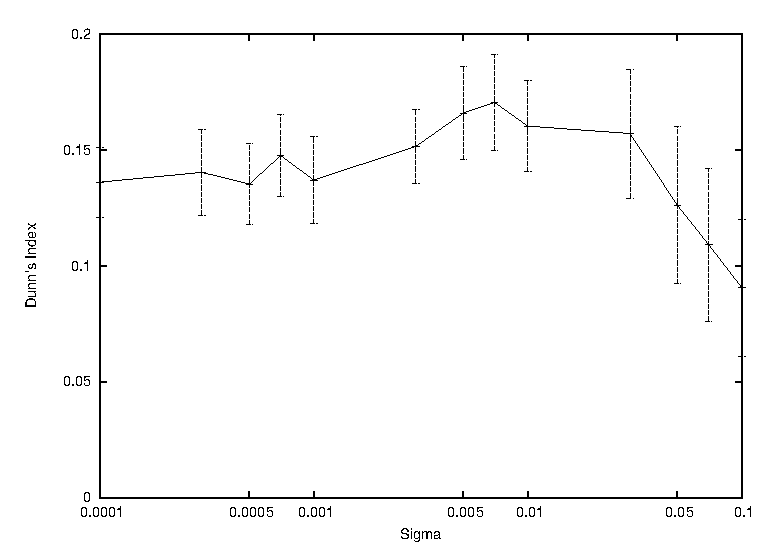
\includegraphics[scale=0.7]{chapter3/stress_ppi_dunn.eps}}
    \subfigure[Microarray $\sigma$ optimization using Davies Bouldin's index]
            {\label{fig:stress_ppi_davies}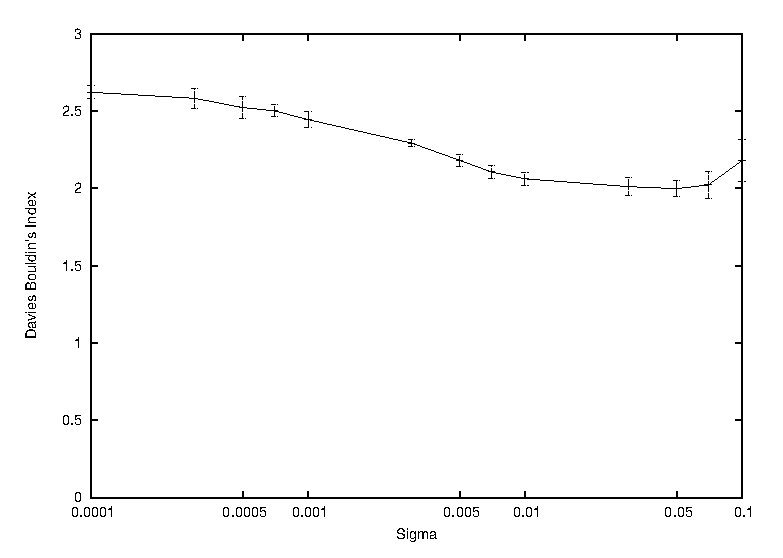
\includegraphics[scale=0.7]{chapter3/stress_ppi_davies.eps}} \\
    \subfigure[PPI $\beta$ optimization using total within-cluster sum of square distances]
            {\label{fig:stress_ppi_withinss}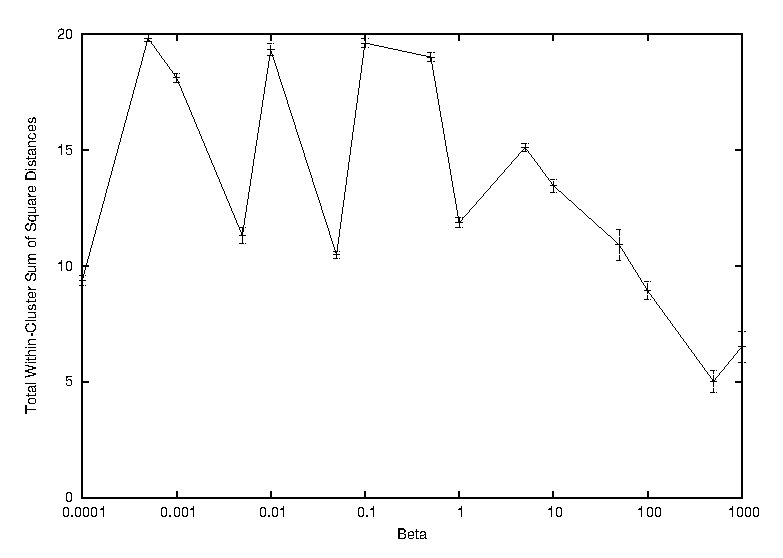
\includegraphics[scale=0.7]{chapter3/stress_ppi_withinss.eps}}
  \end{center}
  \caption{Microarray (stress) and PPI datasets: Sigma and Beta optimization}
  \label{fig:stress_ppi_opt}
\end{figure}

\subsubsection{Stress and ChIP-chip}
For the microarray stress dataset, as seen in Figure-\ref{fig:stress_chip_opt}, the best values in both the Dunn and Davies Bouldin's index graphs is at $\sigma=0.005$. We chose this because of this consensus even though the standard deviation in both cases is quite high. For the ChIP-chip dataset, the \textit{withinss} values have jumped sharply after $\beta=50$. We looked at the diffusion matrix and observed that this was because after $\beta=50$ all the points were being put into few clusters. This is one of the biggest drawbacks of simple measures like \textit{withinss} which unlike Dunn and Davies Bouldin's index does not take cluster separation into consideration. So, out of the remaining smooth region, we picked the value of $\beta=5$ based on it being the lowest.
\begin{figure}[htp]
  \begin{center}
    \subfigure[Microarray $\sigma$ optimization using Dunn' index]
            {\label{fig:stress_chip_dunn}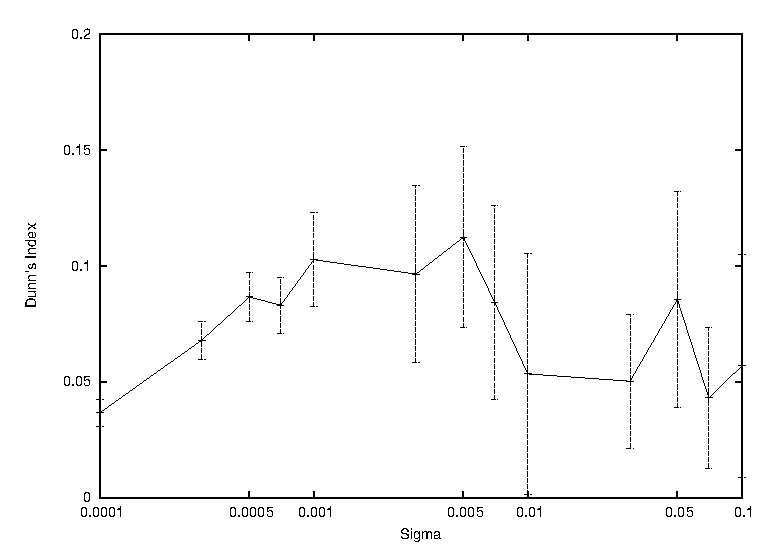
\includegraphics[scale=0.7]{chapter3/stress_chip_dunn.eps}}
    \subfigure[Microarray $\sigma$ optimization using Davies Bouldin's index]
            {\label{fig:stress_chip_davies}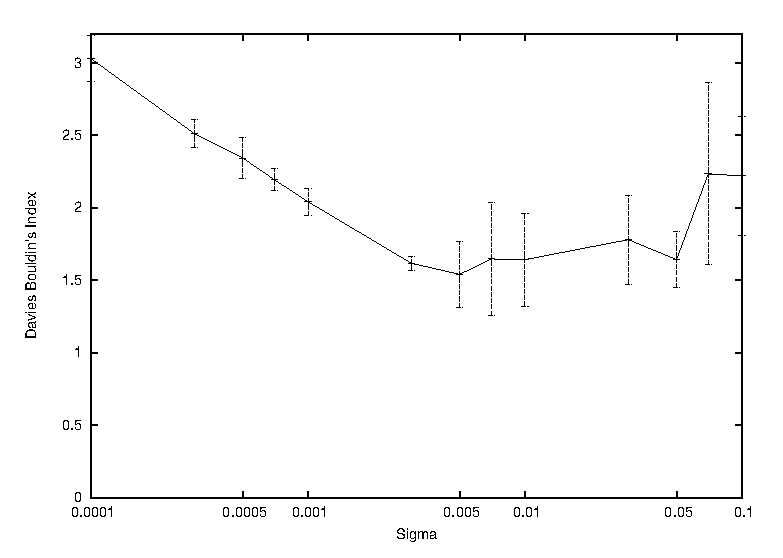
\includegraphics[scale=0.7]{chapter3/stress_chip_davies.eps}} \\
    \subfigure[ChIP-chip $\beta$ optimization using total within-cluster sum of square distances]
            {\label{fig:stress_chip_withinss}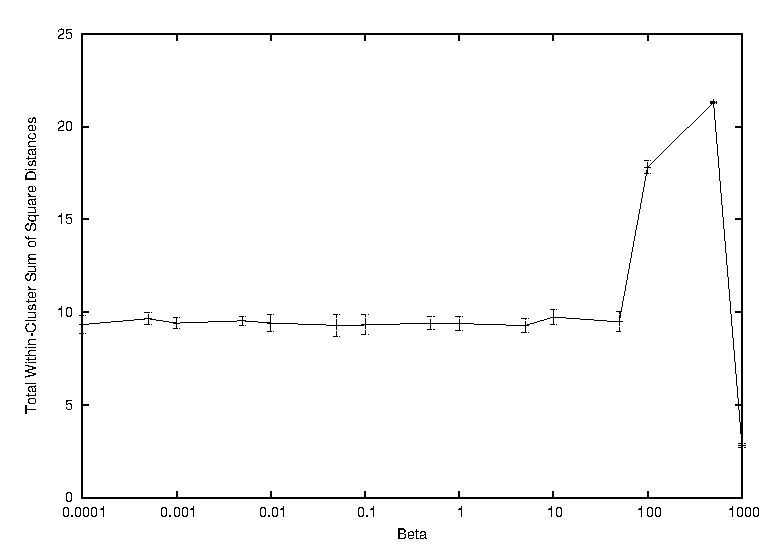
\includegraphics[scale=0.7]{chapter3/stress_chip_withinss.eps}}
  \end{center}
  \caption{Microarray (stress) and ChIP-chip datasets: Sigma and Beta optimization}
  \label{fig:stress_chip_opt}
\end{figure}

\subsubsection{Stress and Yeastract}
Figure-\ref{fig:stress_tf_opt} shows that for the microarray stress dataset, the best values in both the Dunn and Davies Bouldin's index graphs is at $\sigma=0.003$. We chose this because of this consensus. The standard deviation in Dunn index is quite high but its low for Davies Bouldin's index. Again, for the Yeastract dataset, the \textit{withinss} values have jumped sharply after $\beta=10$. We looked at the diffusion matrix and observed that this was because after $\beta=10$ all the points were being put into few clusters as the similarity values were uniformly similar. We chose $\beta=5$ as it was the lowest value in the plot. 
\begin{figure}[htp]
  \begin{center}
    \subfigure[Microarray $\sigma$ optimization using Dunn' index]
            {\label{fig:stress_tf_dunn}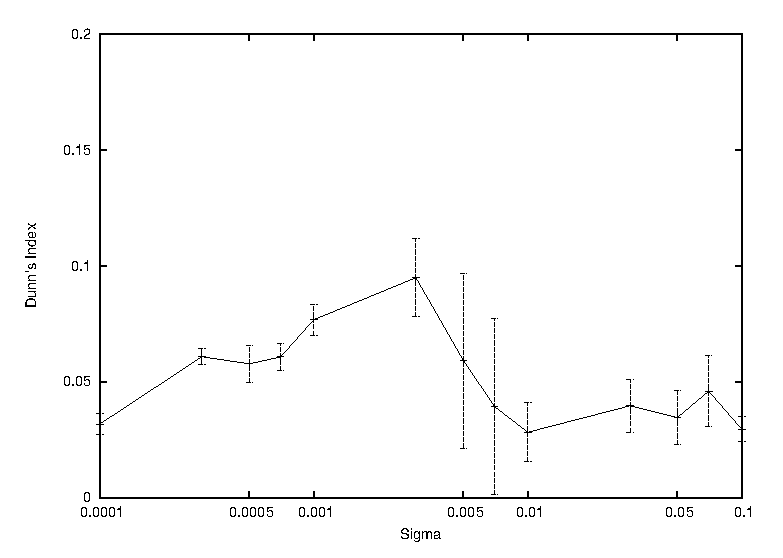
\includegraphics[scale=0.7]{chapter3/stress_tf_dunn.eps}}
    \subfigure[Microarray $\sigma$ optimization using Davies Bouldin's index]
            {\label{fig:stress_tf_davies}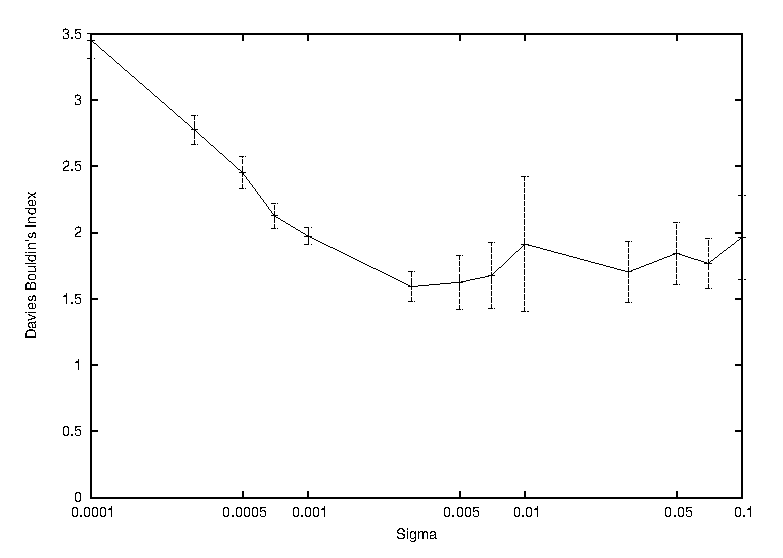
\includegraphics[scale=0.7]{chapter3/stress_tf_davies.eps}} \\
    \subfigure[Yeastract $\beta$ optimization using total within-cluster sum of square distances]
            {\label{fig:stress_tf_withinss}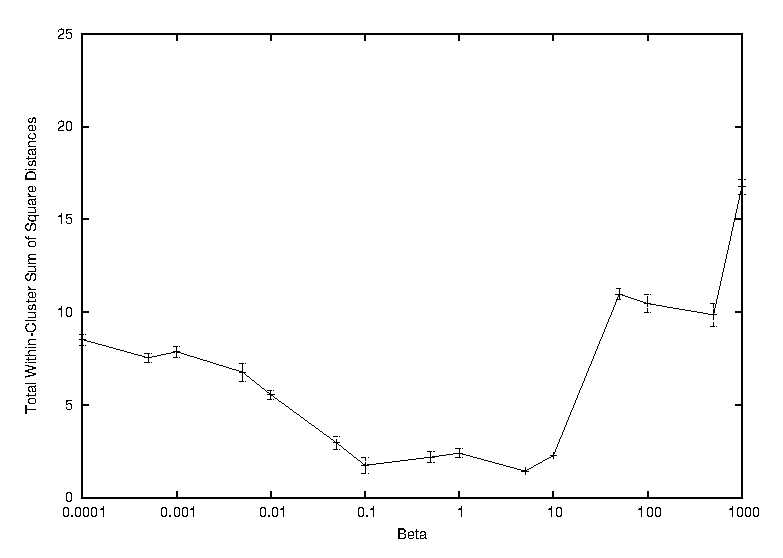
\includegraphics[scale=0.7]{chapter3/stress_tf_withinss.eps}}
  \end{center}
  \caption{Microarray (stress) and Yeastract datasets: Sigma and Beta optimization}
  \label{fig:stress_tf_opt}
\end{figure}

\subsubsection{Cell-cycle and (PPI, ChIP-chip and Yeastract)}
In a similar manner, we found the optimum values for these parameters for the common data between cell-cycle and PPI, Yeastract and ChIP-chip datasets. The plots are in Figures-\ref{fig:ccycle_ppi_opt},\ref{fig:ccycle_chip_opt} and \ref{fig:ccycle_tf_opt} and the parameter choices are summarised in Table-\ref{tab:maxent_mean_pvals}.
\begin{figure}[htp]
  \begin{center}
    \subfigure[Microarray $\sigma$ optimization using Dunn' index]
            {\label{fig:ccycle_ppi_dunn}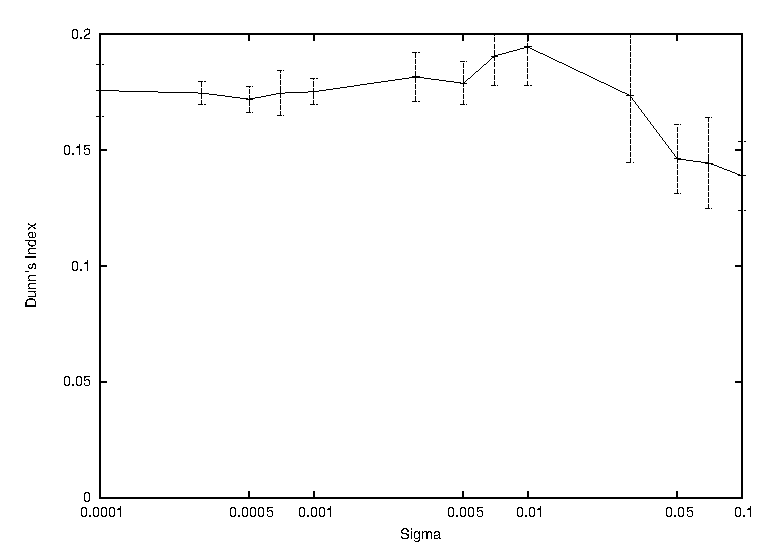
\includegraphics[scale=0.7]{chapter3/ccycle_ppi_dunn.eps}}
    \subfigure[Microarray $\sigma$ optimization using Davies Bouldin's index]
            {\label{fig:ccycle_ppi_davies}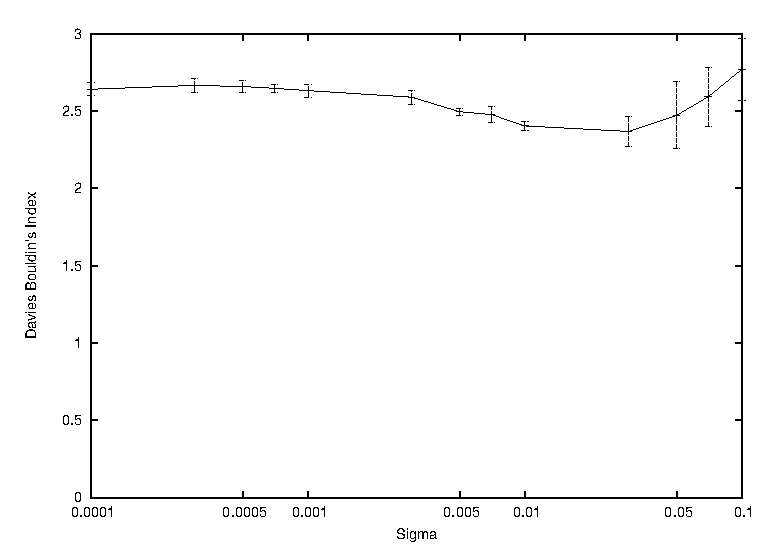
\includegraphics[scale=0.7]{chapter3/ccycle_ppi_davies.eps}} \\
    \subfigure[PPI $\beta$ optimization using total within-cluster sum of square distances]
            {\label{fig:ccycle_ppi_withinss}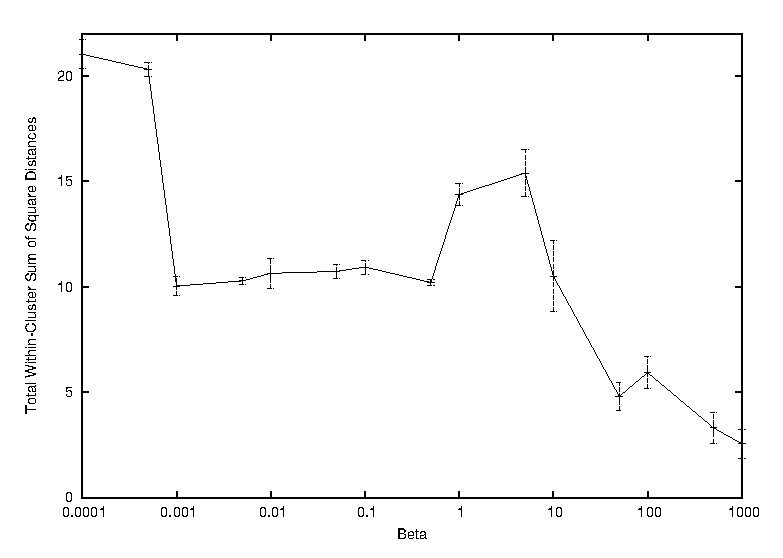
\includegraphics[scale=0.7]{chapter3/ccycle_ppi_withinss.eps}}
  \end{center}
  \caption{Microarray (cell-cycle) and PPI datasets: Sigma and Beta optimization}
  \label{fig:ccycle_ppi_opt}
\end{figure}

\begin{figure}[htp]
  \begin{center}
    \subfigure[Microarray $\sigma$ optimization using Dunn' index]
            {\label{fig:ccycle_chip_dunn}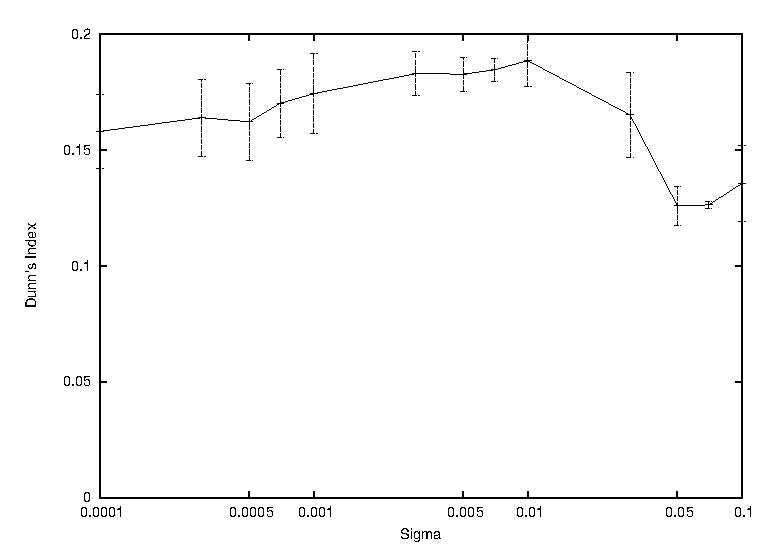
\includegraphics[scale=0.7]{chapter3/ccycle_chip_dunn.eps}}
    \subfigure[Microarray $\sigma$ optimization using Davies Bouldin's index]
            {\label{fig:ccycle_chip_davies}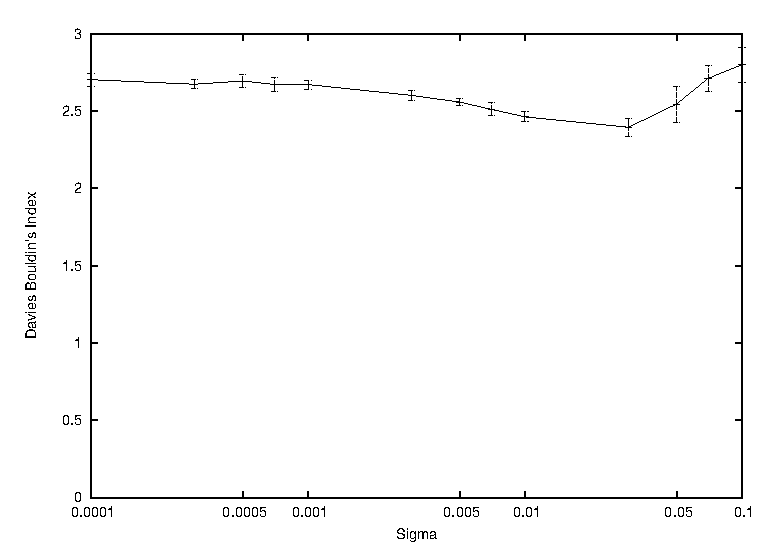
\includegraphics[scale=0.7]{chapter3/ccycle_chip_davies.eps}} \\
    \subfigure[ChIP-chip $\beta$ optimization using total within-cluster sum of square distances]
            {\label{fig:ccycle_chip_withinss}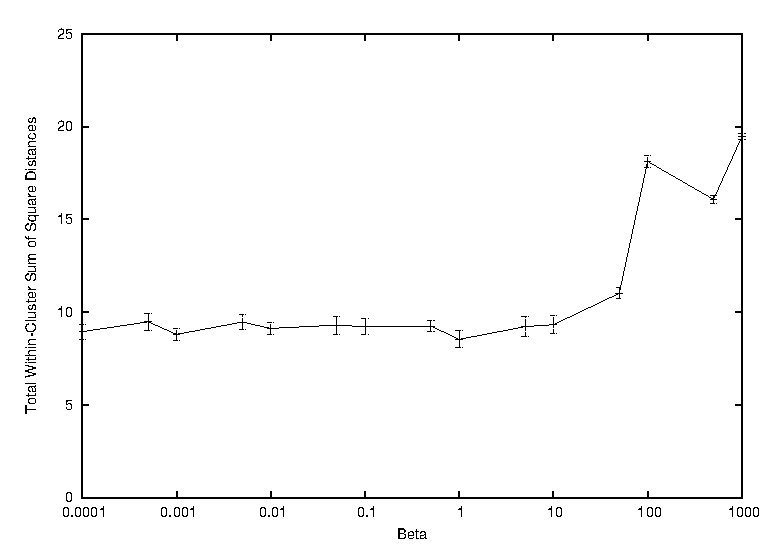
\includegraphics[scale=0.7]{chapter3/ccycle_chip_withinss.eps}}
  \end{center}
  \caption{Microarray (cell-cycle) and ChIP-chip datasets: Sigma and Beta optimization}
  \label{fig:ccycle_chip_opt}
\end{figure}

\begin{figure}[htp]
  \begin{center}
    \subfigure[Microarray $\sigma$ optimization using Dunn' index]
            {\label{fig:ccycle_tf_dunn}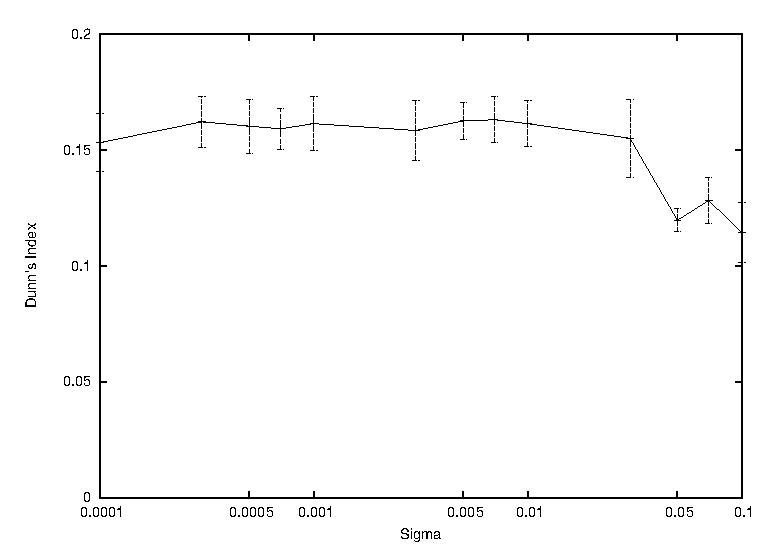
\includegraphics[scale=0.7]{chapter3/ccycle_tf_dunn.eps}}
    \subfigure[Microarray $\sigma$ optimization using Davies Bouldin's index]
            {\label{fig:ccycle_tf_davies}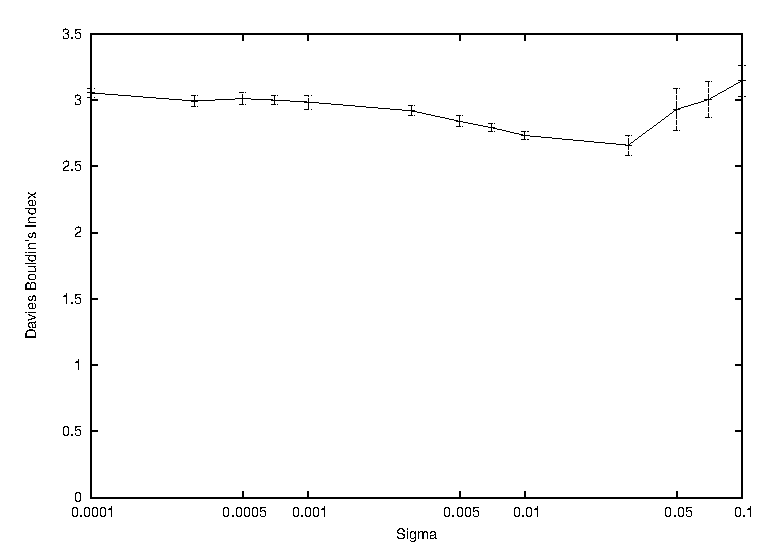
\includegraphics[scale=0.7]{chapter3/ccycle_tf_davies.eps}} \\
    \subfigure[Yeastract $\beta$ optimization using total within-cluster sum of square distances]
            {\label{fig:ccycle_tf_withinss}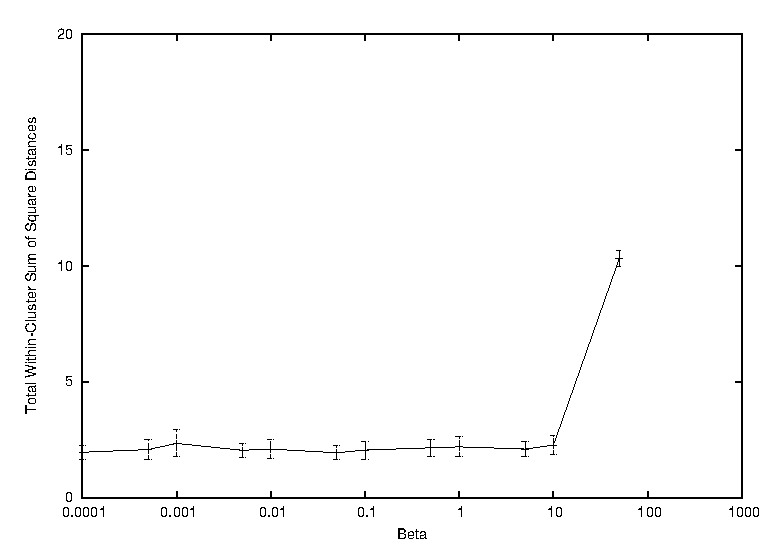
\includegraphics[scale=0.7]{chapter3/ccycle_tf_withinss.eps}}
  \end{center}
  \caption{Microarray (cell-cycle) and Yeastract datasets: Sigma and Beta optimization}
  \label{fig:ccycle_tf_opt}
\end{figure}

\begin{table}[t]
\centering
\begin{tabular}{|c|c|c|}
\hline
Datasets & Sigma & Beta \\
\hline
Stress \& PPI                              & 0.007 & 500 \\ 
Stress \& ChIP-chip                        & 0.005 &  5\\
Stress \& TF-gene interactions (Yeastract) & 0.003 &  5\\
\hline \hline
Cell-cycle \& PPI                              & 0.01 & 1000 \\ 
Cell-cycle \& ChIP-chip                        & 0.01 & 1 \\
Cell-cycle \& TF-gene interactions (Yeastract) & 0.01 & 0.0001 \\
\hline 
\end{tabular}
\caption{Parameter values among pairs of datasets after optimization}
\label{tab:maxent_mean_pvals}
\end{table}
\clearpage

\section{Biological Validation of Results}
\begin{table}[t]
\centering
{\footnotesize
\begin{tabular}{@{\extracolsep{\fill}}|p{0.5in}|p{0.40in}|p{0.50in}|p{0.40in}|p{0.40in}|p{0.40in}||p{0.40in}|p{0.50in}|p{0.40in}|p{0.40in}|p{0.40in}|}
\hline

Datasets & \multicolumn{5}{|c|}{across all terms} & \multicolumn{5}{|c|}{for top 50 terms}\\ \cline{2-11}
       & Dataset A &  Dataset B & MaxEnt Integration & \% Gain for A & \% Gain for B & Dataset A &  Dataset B & MaxEnt Integration & \% Gain for A & \% Gain for B\\
\hline
Stress \& PPI & 6.781  &   10.763     & 8.164  &  20.398  &   -24.14       &  4.177  &  7.203   & 8.012  &  91.793 & 11.23     \\ \hline

Stress \& ChIP-chip & 8.326  & 10.508  & 8.867  &  6.493   & -15.61  &  10.506 & 9.876  & 10.676 &  1.617  & 8.098 \\ \hline

Stress \& Yeastract & 8.924  & 11.876  & 10.346 &  15.929  & -12.88  &  13.363 & 13.855 & 16.379 & 22.575  & 18.220 \\ \hline

\end{tabular}
}
\caption{Stress microarray dataset: Comparison of mean p-values of enriched GO terms before and after maximum entropy data integration}
\label{tab:stress:maxent_mean_pvals}
\end{table}

We follow the same procedure that was followed in the previous chapter (refer Section-\ref{biosig_go}) for biological validation of the resulting clusters. We test each set of clusters obtained after spectral clustering for the enrichment of GO terms. This results in p-values of GO terms in each of the clusters of result. In order to compare two sets of clusters, e.g. before and after data integration, we compute the p-values of GO terms in each of the cluster sets and then report the mean values of negative log of all the p-values of enriched GO terms across all the clusters.

The results of the integration of the stress microarray dataset with ChIP-chip, PPI and Yeastract are in Table-\ref{tab:stress:maxent_mean_pvals}. We have reported percentage gains in GO terms' enrichment before and after integration for each pair of dataset being integrated. Like previous chapter, we have reported the mean results for all the terms as well as top 50 most enriched terms. But, the results are not exactly comparable to the previous chapter. The crucial difference is that there we had used the full set of microarray genes, whereas here we are only using genes that are common across both the datasets which reduces the gene counts considerably as discussed in previous chapter. For each pair of dataset, the first one is referred to as A and the second as B. For example, in the first full row of Table-\ref{tab:stress:maxent_mean_pvals}, stress is referred to as A, while PPI is B. 

The results in Table-\ref{tab:stress:maxent_mean_pvals} clearly indicate that MaxEnt integration has resulted in improvements for the stress datasets with every other dataset. The top 50 term results only accentuate the values for PPI and Yeastract. However, when we observe if the non-microarray dataset had gained much from the integration, the results for all the terms indicate negative results while the top 50 terms indicate positive results. As observed in the last chapter, this could be because of the removal of the noisier terms when we only select the top 50 terms.

\begin{table}[t]
\centering
{\footnotesize
\begin{tabular}{@{\extracolsep{\fill}}|p{0.5in}|p{0.40in}|p{0.50in}|p{0.40in}|p{0.40in}|p{0.40in}||p{0.40in}|p{0.50in}|p{0.40in}|p{0.40in}|p{0.40in}|}
\hline

Datasets & \multicolumn{5}{|c|}{across all terms} & \multicolumn{5}{|c|}{for top 50 terms}\\ \cline{2-11}
       & Dataset A &  Dataset B & MaxEnt Integration & \% Gain for A & \% Gain for B & Dataset A &  Dataset B & MaxEnt Integration & \% Gain for A & \% Gain for B\\
\hline
Cell-Cycle \& PPI       & 6.651  & 6.151  & 6.588  &  -0.960 & 7.103  & 4.795 & 6.019  &  6.582 &  37.270  & 9.355 \\ \hline
 
Cell-Cycle \& ChIP-chip & 7.069  & 6.069  & 6.794  & -3.883  & 11.945 & 8.036 & 6.390  &  6.795 &  -15.44  & 6.346 \\ \hline

Cell-Cycle \& Yeastract & 7.584  & 5.988  & 7.222  &  -4.776 & 20.615 & 10.059 & 6.894 & 9.298  & -7.570 & 34.869 \\ \hline	

\end{tabular}
}

\caption{Cell-cycle microarray dataset: Comparison of mean p-values of enriched GO terms before and after maximum entropy data integration}
\label{tab:ccycle:maxent_mean_pvals}
\end{table}

For the cell-cycle dataset, the results are very different. Here, the cell-cycle dataset does not show any improvement except with PPI (for top 50 terms). On, the other hand, rest of the datasets have shown improvement when merged with the cell-cycle dataset. As we discussed earlier that this technique merges two datasets by taking their dominant eigenvectors. In the case of stress dataset, both the datasets gained biological significance whereas now cell-cycle is always the loser. The PPI, Yeastract are both curated datasets. Most of the curated datasets are taken from experiments that are conducted in non-stress environments to study the regular activities of genes. Therefore, they are more similar to the cell-cycle dataset. We had observed this in the last chapter where cell-cycle dataset showed much better gains with PPI and Yeastract constraints as compared to the stress dataset. Because of this similarity, the cell-cycle dataset has not gained much from the others. In case of stress, they were very dissimilar and hence both gained information from each other which led to improvement in their scores.    
\begin{figure}
\begin{center}
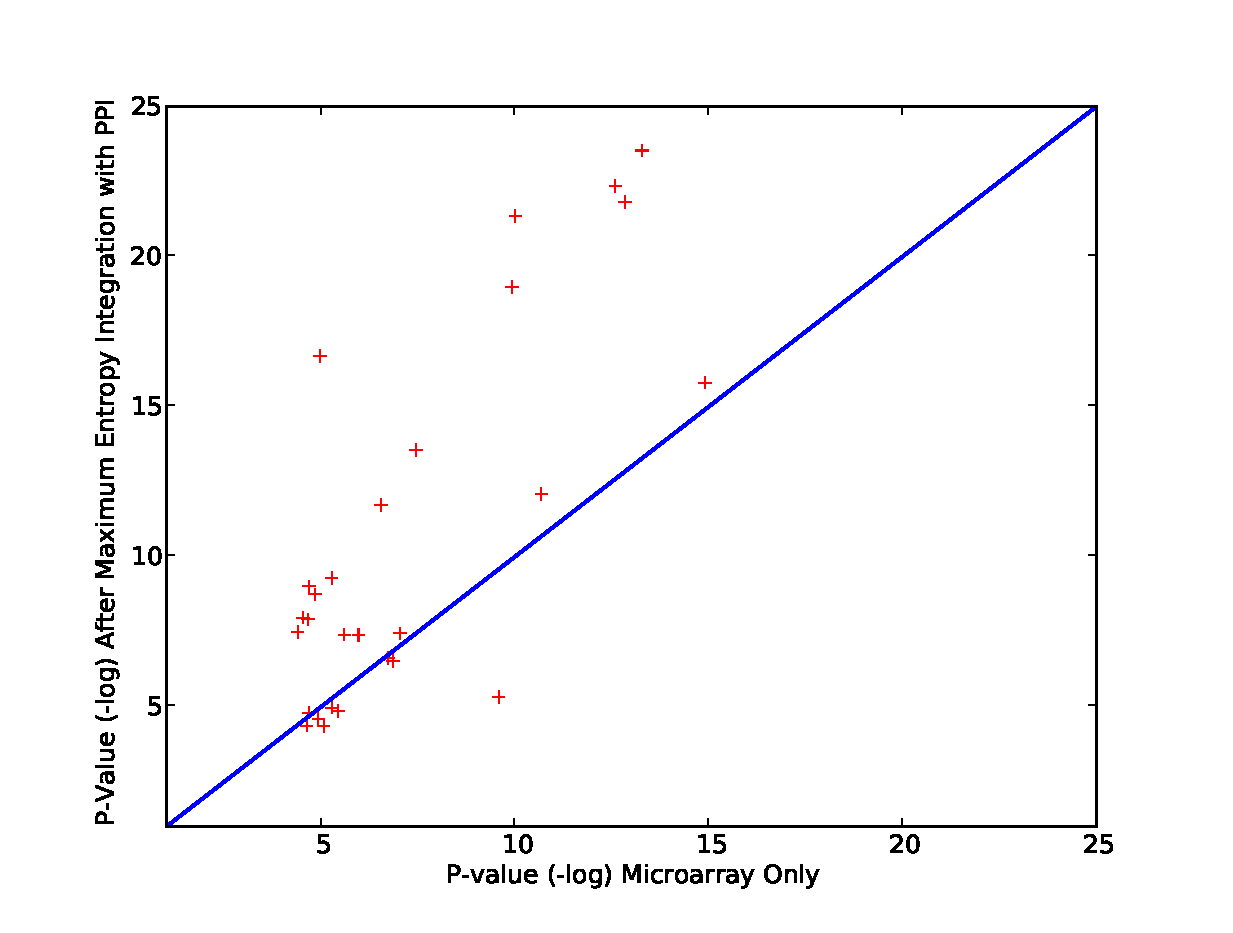
\includegraphics[scale=0.55]{chapter3/stress_ppi_maxent.eps}
\end{center}    
\caption{Comparison of biological significance before and after maximum entropy integration of stress microarray and PPI datasets}
\label{fig:maxent_biol_valid}
\end{figure}

Figure-\ref{fig:maxent_biol_valid} shows the change in p-values of individual GO terms before and after the integration of PPI data with the stress microarray data, the integration that had shown maximum percentage gain. The x-axis indicates the GO term values before the integration (microarray only) while the y-axis is those of after integration (microarray + PPI data). If there was no effect of data integration then the values would have perfectly aligned on the diagonal. The further away they are from the diagonal (vertically) on either side of the diagonal, the more enriched they are on that side (below the diagonal for before integration and above the diagonal for after integration). For the stress dataset, we can clearly see in Figure-\ref{fig:maxent_biol_valid} that there are many more terms that are better enriched after the integration. 

All our result data is available upon request. For the the best clustering gain results (top 50 terms) across both the datasets (maximum entropy integration of stress and PPI dataset), we have provided the best 5 enriched GO terms in each cluster in Table-\ref{appendix:maxent_stress_pval} as part of Appendix-\ref{appendix:go_enrichment_results}. 
\section{Related Work and Discussion}

Combining evidence from multiple biological datasets is not a new phenomenon. Earlier efforts in this direction related to clustering were classified under co-clustering. In this technique, the datasets are combined by assigning equal or varying weights to each dataset. For distance based clustering techniques, individual distances derived from each datasets are merged in order to come up with a new one which is then used for clustering. \citet{Hanisch2002Coclustering} proposed a distance metric that combines information from expression data and biological networks and uses it for clustering genes. They define a graph distance function on a metabolic network derived from MIPS \citep{Gueldener2006MPact} and combine it with a correlation-based distance function for microarray gene expression measurements. They assigned equal weights to both the sources and then used the resulting distance for hierarchical clustering. They show that their technique was able to find biologically meaningful clusters. \citet{huang2006incorporating} developed a similar algorithm in which instead of combining the two information sources with equal weights, they used a \textit{shrinkage} approach with the genes belonging to the same functional classes assigned zero distance (maximal similarity) and the rest of the genes using the distance calculated from the microarray data. This is then used for K-medoids clustering on simulated data as well as real one for gene function prediction. \citet{bramier2007coclustering} proposed co-clustering based on a combined distance metric from microarray gene expression data and Gene Ontology terms for \ac{SOM}. Apart from distance based clustering, various researchers have combined datasets using model based clustering as well \citep{pan06incorporating}.

Kernel integration has been used in the field of supervised learning in order to combine kernels from different datasets. \citet{Holloway2006MachineLearning} used it for predicting the TF binding locations on DNA. They have used 18 different datasets - both sequence and non-sequence (expression, GO) and calculated kernels from them. The goal was to combine the kernels and then use the final combination in \ac{SVM} for classification. They have used each kernel individually and calculated the \textit{F statistic} (a widely used measure for performance of a classifier). In order to combine the kernels, these F values were used as weights for each of the kernel. One of the drawbacks is that the F-statistic does not take into account the relationship of the variables but only a macro view of the performace of the whole kernel encoding. They reported that combining all datasets resulted in 73\% coverage of known interactions. 

A more mathematically sound approach to kernel integration was developed by \citet{lanck04kerneldatafusion}. They have formulated the optimization problem as a convex optimization problem and then used \ac{SDP} to solve it. The technique is both statistically sound and computationally efficient. They used this technique in order to classify different classes of proteins (membrane vs ribosomal) using kernels derived from protein sequence, microarray expression and protein-protein interaction data. They have reported an improvement in the classification results when the kernels are combined as compared to individual kernels. The biggest drawback of such techniques is that the weights that are assigned to each dataset do not take into account the correlation between different variables across datasets and assigns one common weight for the whole dataset. Our technique tries to solve it by picking only the highest eigenvectors.

\citet{lewis06svm} did an investigation of weighted and unweighted kernel combination in classifying GO terms associated with protein sequences using SVM. They came to the interesting conclusion that for this particular task, unweighted combination of kernels is better than weighted ones. In order to compute the weights they too have used the SDP technique. \citet{Liang2008Adaptive} developed a technique to learn an optimal diffusion kernel as a convex combination of many kernels constructed from biological networks and then used the optimal kernel for protein function prediction. They report superior performance for the combined kernel in comparison to individual kernels. 

Most of the above kernel combination techniques are based on \textit{supervised learning} and the individual kernel weights are optimized using some training data. But Kernel integration in an unsupervised setting (when training data is unavailable) is hard because we have no way to compute the individual weights. 

\citet{Tsuda2004Learning} used a very different approach to guess a kernel matrix from incomplete data. The underlying approach is that some values in the matrix are known and they try to fill in the rest so that the resulting matrix has maximum possible entropy. They used this to compute kernels from PPI data and metabolic network and used these for the classification task and report that the maximum entropy kernel beats the diffusion kernel in classification accuracy. \citet{fujibuchi2007classification} have used the maximum entropy devised by \citet{Tsuda2004Learning} and applied it on three microarray datasets (heterogeneous kidney carcinoma, noise introduced leukemia and hetergenous oral cavity carcinoma metastasis) for the purpose of evaluating its classification performance as compared to single kernels (linear, polynomial and rbf). They report better overall performance for the maximum entropy kernel compared to others in classification performance.  

In practise, the principle of maximum entropy is useful when applied to verifiable information. A piece of information is verifiable if it can be determined whether a given distribution is consistent with it. Given this information, the maximum entropy procedure consists of seeking the probability distribution which maximizes information entropy, subject to the constraints of the information. This constrained optimization problem is typically solved using the method of Lagrange multipliers. Both these approaches to kernel approximation \citep{Tsuda2004Learning, fujibuchi2007classification} using maximum entropy is based on maximising the entropy subject to certain constraints. However, this is very different from our approach where we do not treat it as a entropy maximisation subject to certain constraints. We try to assume a distribution with maximum entropy as the ideal distribution when no other information is available in order to combine the similarity matrices. So, when we have multiple sets of evidence, e.g. PPI and microarray data, we try to combine them through their similarity matrices such that the resulting distribution (of the combined similarity matrix) has the maximum entropy.

The ideal scenario of its use is where one of the datasets is a very noisy sample while the other one is a \textit{compendium} or reference dataset collected over time from various sources. The compendium acts as an average of all known observations, which when combined using this technique with the sample, fills in the eigenvalues about which the sample dataset is most \textit{confused} about. So, the sample dataset gets to keep all its prominent eigenvalues while borrowing ones from the compendium about which it is not so confident. 


\section{Conclusion}

We have proposed a technique to integrate two diverse datasets where one is available in the form of vectorial data while the other is available in the form of a graph. The core idea is based on work done by \citet{thomaz2004covariance}. While they had used it to combine covariance matrices where one of them is singular, we have extended its use to general kernel combination after observing the similarities between the properties of a covariance matrix and a similarity matrix obtained using a kernel function. 

Integrating such diverse datasets is not possible unless we resort to some kind of normalization. We have used similarity functions to compute similarity matrices for these datasets as the \textit{normalization} step. We have used the same techniques that we used in the previous chapter in order to compute the similarity function parameters.
 
While in the supervised setting we have an objective function that we can use to optimize the contribution of each of the similarity functions, in an unsupervised setting there is no such facility. Hence, most previous works have used ad-hoc techniques in order to integrate different datasets. We argue that under such a setting when no further evidence is available to assign weights to individual datasets then the \textit{principle of maximum entropy} is the most natural and valid choice. Apart from conceptual elegance, other benefits of this technique are that no time consuming optimization is required to search for contributions of each dataset and fairly simple and intuitive linear algebra computations are needed. Since our technique is quite generic, in future, our work can be extended to integrating other sources of data, for example  the similarity between the promoter sequences of genes.  

One of the key shortcomings for the biological validation of our results is that it is not possible to get datasets that were generated on the same strains under similar experimental conditions. Both our datasets were compiled by independent researchers. When datasets that are generated under similar conditions start becoming available we would be more confident in assessing the biological significance of the results.

There is no gold-standard for validating the clusters and there are no reference datasets on which we can compare the results with other techniques. Gene ontology while being one of the more informative sources of validation is still an indirect validation technique. Also, there is a fundamental limitation of the underlying experimental techniques, since microarrays themselves do not represent a single time point, but rather the integration of gene activity over a time period. 